\documentclass[a4paper, 12pt]{article}
\usepackage[total={17cm,25cm}, top=2.5cm, left=2.5cm, right=2.5cm,  includefoot]{geometry}
\usepackage[utf8]{inputenc}
\usepackage{array}
\usepackage{multirow}
\usepackage{hhline}
\usepackage{gensymb}
\usepackage{graphicx}
\graphicspath{ {} }
\usepackage[czech]{babel}
\usepackage{enumitem}
\usepackage{pdfpages}
\usepackage{amsmath}
\usepackage{verbatim}
\usepackage{listings}
\usepackage{hyperref}
\usepackage{amssymb}


\pagestyle{empty} % vypne číslování stránek




\usepackage[OT2,OT1]{fontenc}
\newcommand\cyr
{
\renewcommand\rmdefault{wncyr}
\renewcommand\sfdefault{wncyss}
\renewcommand\encodingdefault{OT2}
\normalfont
\selectfont
}
\DeclareTextFontCommand{\textcyr}{\cyr}
\def\cprime{\char"7E }
\def\cdprime{\char"7F }
\def\eoborotnoye{\char’013}
\def\Eoborotnoye{\char’003}


\begin{document}



\begin{titlepage}
\begin{center}
\noindent
\Large \textbf{České vysoké učení technické v Praze }\\ Fakulta stavební
\vspace{5cm}

\huge

%vložení loga cvut
\begin{figure}[h!]
	\centering
	
\includegraphics[width=7cm]{logo.png}
\end{figure}

\vspace{0.5cm}

Algoritmy v digitální kartografii \\

\vspace{3cm}

\Huge  
Konvexní obálky\\

\vspace{2cm}

\Large
Bc. Petra Pasovská \\
Bc. David Zahradník \\

\end{center}

\end{titlepage}




\pagestyle{plain}     % zapne obyčejné číslování
\setcounter{page}{1}  % nastaví čítač stránek znovu od jedné

\tableofcontents
\newpage

\section{Zadání}
Níže uvedené zadání je kopie ze stránek předmětu. 

\begin{figure}[h!]
	\centering
	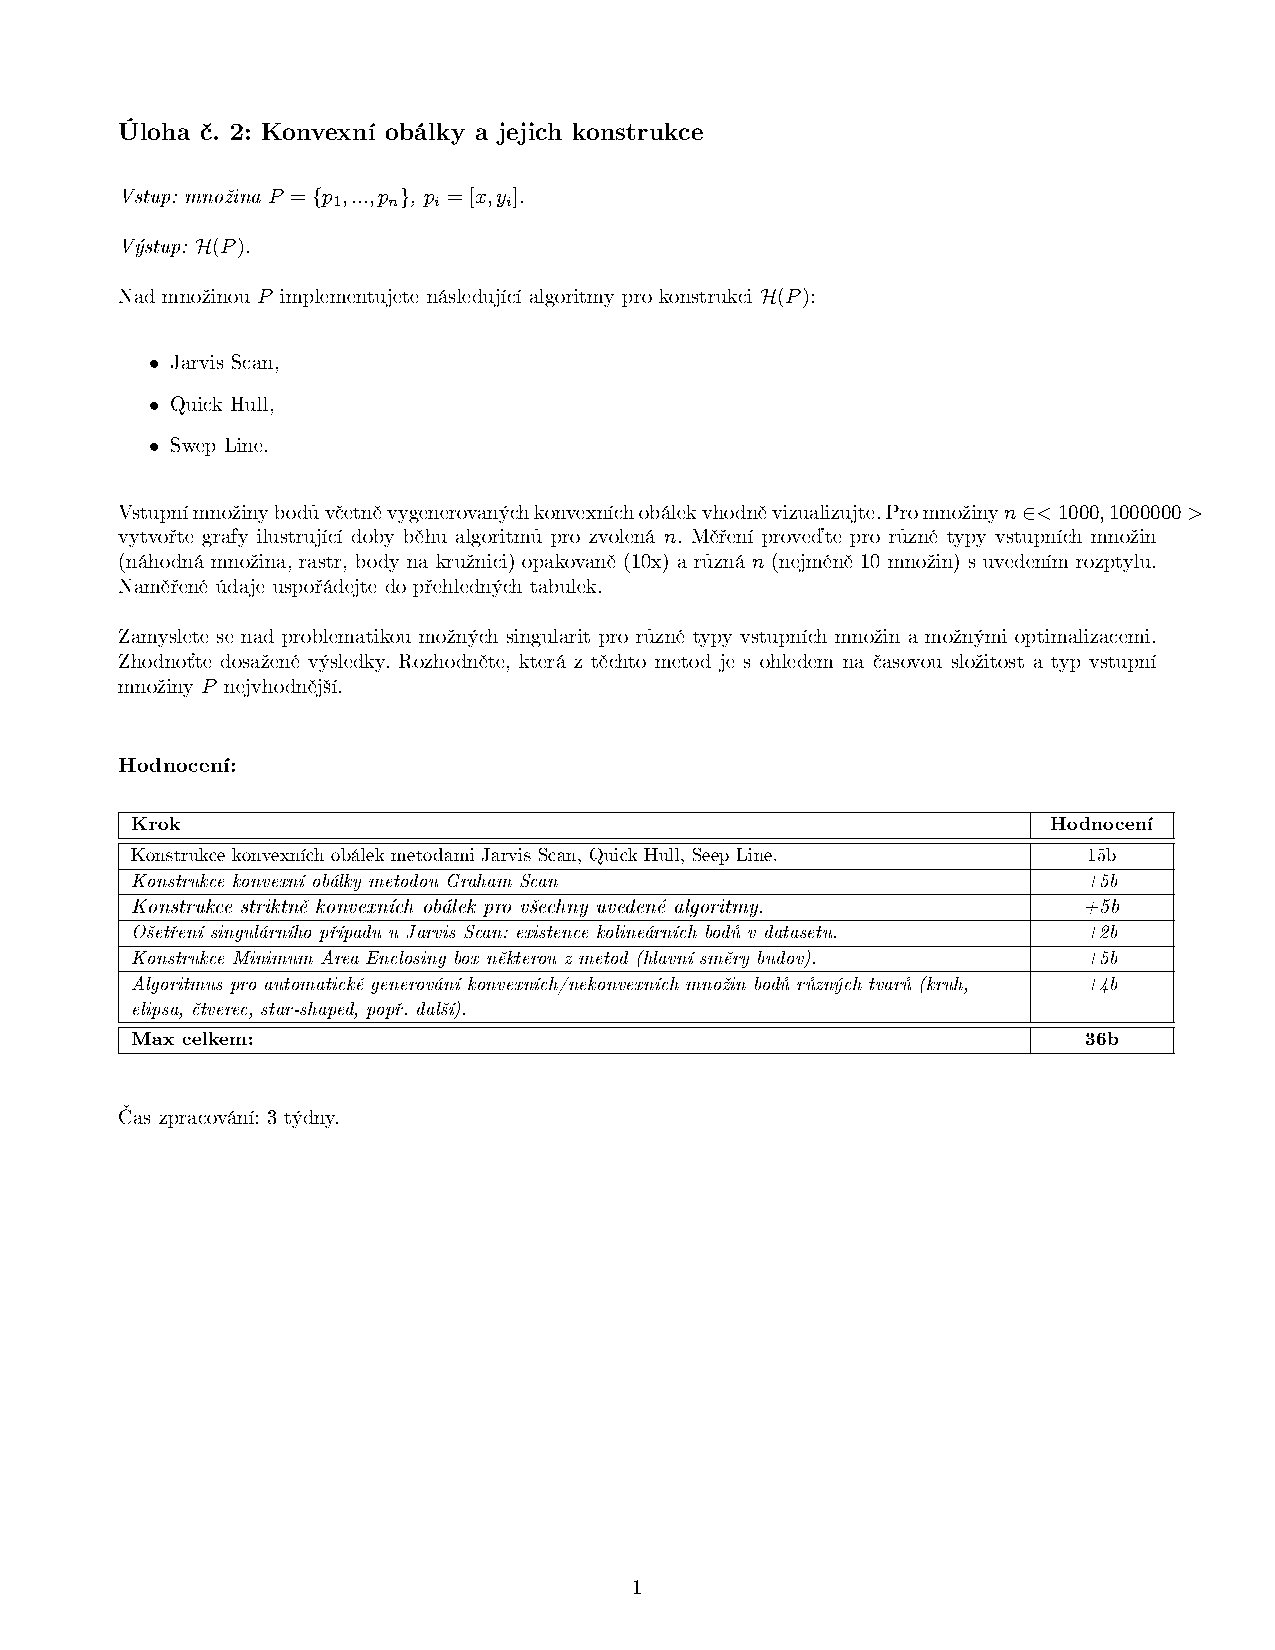
\includegraphics[clip, trim=0cm 10cm 0cm 3cm, width=1.2\textwidth]{zadani.pdf}
\end{figure}

\subsection{Údaje o bonusových úlohách}
Z bonusových úloh byl vytvořen algoritmus pro automatické generování množin bodů různých tvarů. Uživatel si může v aplikaci sám zvolit, zda chce vygenerovat kruh, elipsu, čtverec, star-shaped či grid. Byla vložena i možnost náhodného rozmístění bodů v daném zobrazovacím okně. Dále byl vytvořen algoritmus pro výpočet konvexní obálky metodou Graham Scan. V rámci aplikace je i fungující výpočet konstrukce Minimum Area Enclosing Box. V neposlední řadě byly všechny vytvořené konvexní obálky zredukovány tak, aby vytvářely striktně konvexní obálky.


\clearpage

\section{Popis a rozbor problému}
Hlavním cílem této úlohy je tvorba aplikace, která pro vygenerované množství bodů vytvoří konvexní obálku za pomoci různých algoritmů. Pro jednotlivé metody byla zapisována i doba trvání algoritmu. Výsledné časy jsou v závěru následně porovnány.\\
\\
Lze říci, že konvexní obálka množiny M je nejmenší konvexní množina, která množinu M obsahuje. V současné době mají konvexní obálky, v některých literaturách označovány jako konvexní obaly, mnoho využití. Často se využívají jako první odhad tvaru nějakého prostorového jevu, např. detekce kolizí, detekce natočení budov a jejich tvaru v kartografii, analýza shluků atd. [Zdroj: 1]
\\

\begin{figure}[h!]
	\centering
	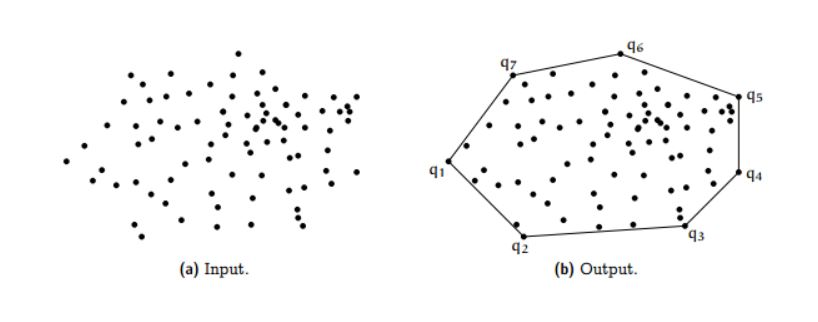
\includegraphics[width=9cm]{convex_hull.jpg}
	\caption{Ukázka vstupních bodů, kolem nichž je vytvořena konvexní obálka. [zdroj: 2]}
\end{figure}

Konvexní obálky využívá celá řada vědních oborů. Zajímavé bylo využití konvexních obálek v paleontologii, kde za pomoci konvexních obálek jsou vědci schopni určit přibližně tvar těla vyhynulých živočichů, jejichž kosti byly nalezeny. \\

\begin{figure}[h!]
	\centering
	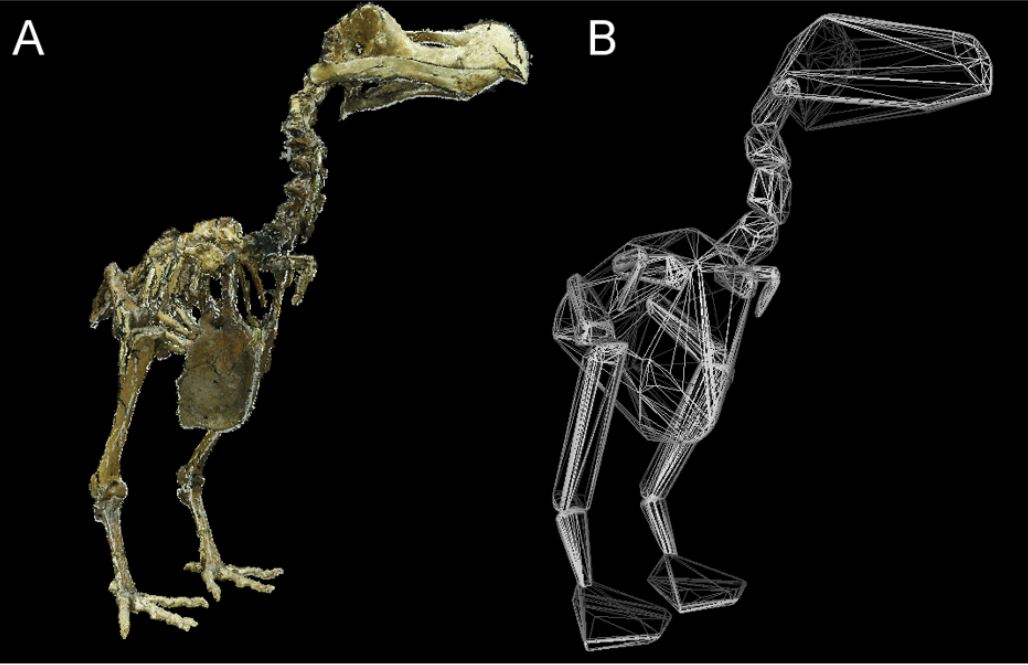
\includegraphics[width=10cm]{paleontology.jpg}
	\caption{Využití konvexních obálek v paleontologii [zdroj: 3]}
\end{figure}


\section{Popis použitých algoritmů}
Existuje několik způsobů jak vytvořit konvexní obálku. V této úloze byly použity pro tovrbu 4 metody - Jarvis Scan, Quick Hull, Sweep Line a Graham Scan.

\subsection{Jarvis Scan}
Tato metoda bývá přirovnávána ke způsobu balení dárků (alternativní název Gift Wrapping Algorithm). Předpokladem pro algoritmus Jarvis Scan je, že 3 body nesmí ležet na jedné přímce. Metoda je poměrně snadná pro zápis, velkou nevýhodou je však časová náročnost O($n^2$), které lze dosáhnout, pokud body z množiny S leží na kružnici. Běžný čas výpočtu bývá O(n*h), kde n je počet vstupních bodů a h je počet bodů, které tvoří obálku. [zdroj: 1]\\
\\
Metoda je pojmenována po R. A. Jarvisu, který ji publikoval v roce 1973. \\
\\
Abychom byli schopni algoritmus sestavit, je potřeba nalézt pivot, označme jej q. Nalezení pivota má časovou náročnost O(n). Pivota nalezneme jako bod s minimální hodnotou souřadnice Y. Následně porovnáváme úhel, který svírá pivot a bod následující a předcházející pivotu, dokud nenalezneme maximální úhel. Když takovýto úhel nalezeneme, je přidán mezi body konvexní obálky. V algoritmu dojde k přeindexování bodů a jsou porovnávány následující body, dokud nově vložený bod není pivot. 

\begin{figure}[h!]
	\centering
	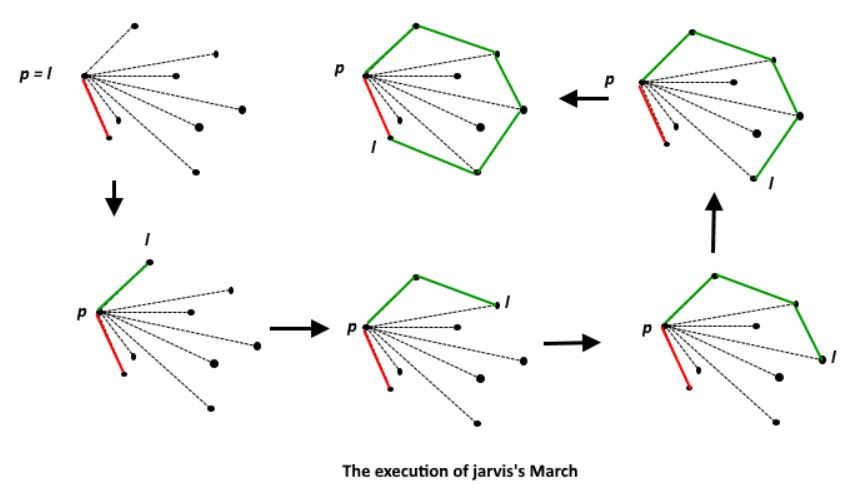
\includegraphics[width=10cm]{jarvis.jpg}
	\caption{Princip Jarvis Scan algoritmu [zdroj: 4]}
\end{figure}

\subsubsection{Problematické situace}
K chybě v algoritmu může dojít v případě, že tři body budou kolineární. Tedy v případě, že se budou tři následující body nacházet na jedné přímce:  $ p_i, p_{i+1}, p_{i+2} \in \vec{x} $.
\\
napsat řešení 



\subsubsection{Implementace metody}
\begin{enumerate}
\item Nalezení pivota q:  $ q = min(y_i) $ 
\item Přidej bod q do konvexní obálky:  $ q \rightarrow H  $ 
\item Inicializuj: $p_j = q; p_{j+1} = p_{j-1}$
\item Opakuj, dokud: $ p_{j+1} \ne q $
\subitem Nalezni $p_{j+1}$: $ p_{j+1} = arg  max_{\forall p_i \in P}  \angle (p_{j-1}, p_j, p_i)$
\subitem Přidej $p_{j+1}$: $ p_{j+1} \rightarrow H  $
\subitem Přeindexování bodů: $ p_{j-1} = p_j; p_j = p_{j+1}  $
\end{enumerate}

\subsection{Quick Hull}
Metoda Quick Hull slouží k vytvoření konvexní obálky nad konečným počtem bodů. Využívá techniku "Rozděl a panuj", označovanou anglicky "Divide and Conquer". V této metodě lze najít analogii s QuickSortem, odkud také pochází označení algoritmu. Jedná se o poměrně rychlý algoritmus, časová náročnost je O(n*log(n)), v nejhorším případě je však časová náročnost kvadratická O($n^2$). \\

Pro výpočet metodou Quick Hull je nejprve zapotřebí nalézt extrémní body, v aplikaci byly souřadnice setříděny podle x-ové souřadnice. Bod s nejnižší a nejvyšší hodnotou x-ové souřadnice je vložen do množiny, do které uchováváme body konvexní obálky. Těmito body je vedena pomyslná přímka, která množinu bodů rozdělí na dvě množiny - horní a dolní. V každé polorovině nalezneme nejvzdálenější bod od přímky, tento bod přidáme do množiny bodů patřících do konvexní obálky a vytvoříme přímky tohoto bodu a krajních bodů předešlé přímky. Následně pokračujeme analogicky a nad každou nově vzniklou přímkou nalezneme nejvzdálenější bod.

\begin{figure}[h!]
	\centering
	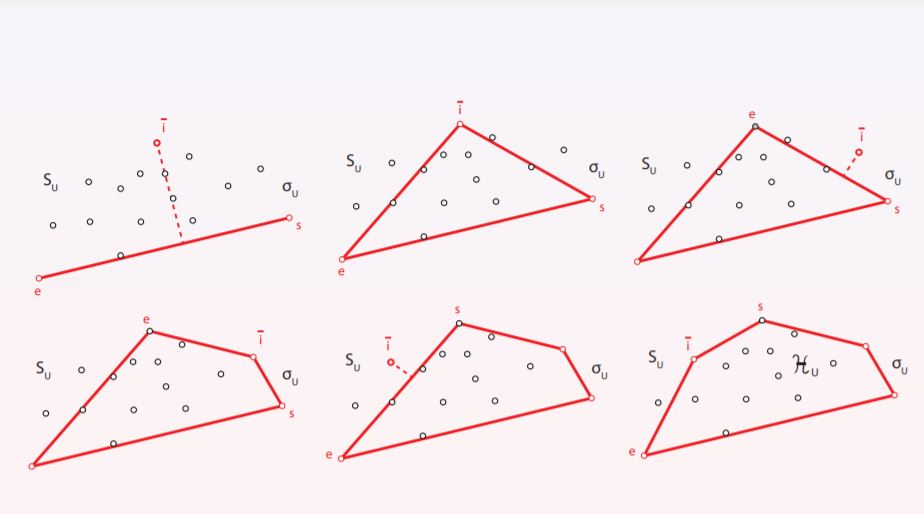
\includegraphics[width=10cm]{quickhull.jpg}
	\caption{Princip Quick Hull algoritmu [zdroj: 5]}
\end{figure}

\subsubsection{Implementace globální metody}
\begin{enumerate}
\item Vytvoření množiny konvexní obálky, horní a dolní množiny:  $H = 0; S_U = 0; S_L = 0 $ 
\item Nalezení extrémních hodnot:  $ q_1 =  min_{\forall p_i \in S}(x_i); q_3 =  max_{\forall p_i \in S}(x_i) $ 
\item Přidání extrémních bodů do horní a dolní množiny: $S_U \leftarrow q_1; S_U \leftarrow q_3; S_L \leftarrow q_1; S_L \leftarrow q_3 $
\item Pro všechny body množiny: $\forall p_i \in S  $
\subitem Rozhodnutí, zda bod patří do horní množiny: $ if(p_i \in \sigma_l(q_1, q_3)) S_U \leftarrow p_i  $
\subitem V opačném případě: $ S_L \leftarrow p_i  $
\item Přidání krajního bodu do konvexní obálky: $H \leftarrow q_3$
\item Nalezení nejvzdálenějšího bodu $c$ v horní části od přímky, přidání do množiny konvexní obálky a opakování vůči nově vzniklé přímce.
\item Přidání krajního bodu do konvexní obálky: $H \leftarrow q_1$
\item Opakování hledání nejvzdálenějšího bodu v dolní části.
\end{enumerate}

Tady nevím, jestli nerozepsat i implementaci lokální metody??? Možná by to pak bylo pochopitelnější


\subsection{Sweep line}
Metoda Sweep line, v češtině označovaná také jako metoda zametací přímky, využívá strategii inkrementální konstrukce. Množinu bodů si v dané dimenzi rozdělíme na zpracovanou a nezpracovanou část. Rozdělovací kritérium je ve většině případů jedna ze souřadnicových os. Je zde tedy nutné body podle této osy seřadit a následně vyhodnocovat každý následující nezpracovaný bod. Body se vyhodnocují v závislosti na jejich poloze vůči tečně. Časová složitost této metody je O(n log(n)). 

\begin{figure}[h!]
	\centering
	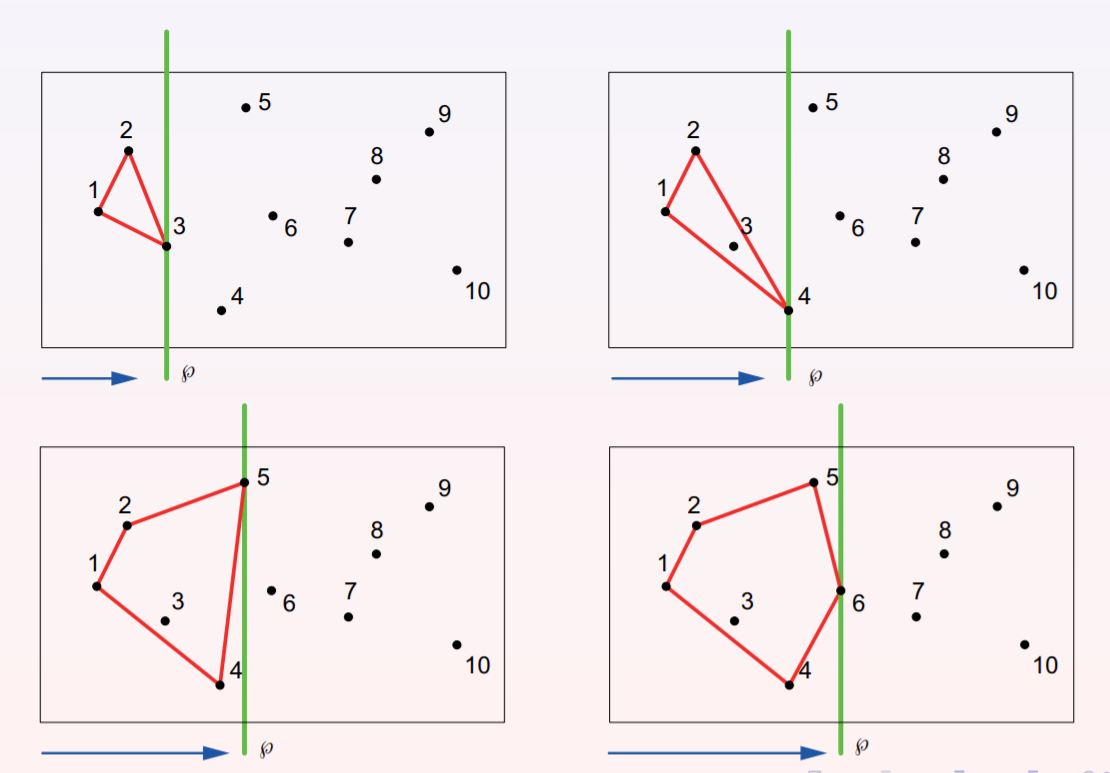
\includegraphics[width=10cm]{sweep_line.jpg}
	\caption{Princip algoritmu zametací přímky [zdroj: 5]}
\end{figure}

\subsubsection{Implementace metody}
\begin{enumerate}
\item Seřazení bodů množiny podle osy x: $ Sort P_s = sort(P) by x $ 
\item Vyhodnocení v případě, že bod $p_3$ leží v levé polorovině od přímky$ p_1, p_2$:  $ if (p_3 \in \sigma_L (p_1, p_2)) $ 
\subitem Změna indexů následovníků: $ n[1] = 2; n[2] = 3; n[3] = 1  $
\subitem Změna indexů předchůdců: $ p[1] = 3; p[2] = 1; p[3] = 2  $
\item Vyhodnocení v případě, že bod$ p_3$ leží v levé polorovině od přímky$ p_1, p_2$:  $ if (p_3 \in \sigma_P (p_1, p_2)) $ 
\subitem Změna indexů následovníků: $ n[1] = 3; n[3] = 2; n[2] = 1  $
\subitem Změna indexů předchůdců: $ p[1] = 2; p[3] = 1; p[2] = 3  $
\item Vyhodnocování následujících bodů: $ for  p_i \in P_S, i \textgreater 3$
\subitem Porovnání hodnoty souřadnice y: $ if (y_i \textgreater y_{i-1})  $
\subsubitem Změna indexů při splnění podmínky: $ p[i] = i-1; n[i] = n[i-1]$
\subsubitem V opačném případě: $ p[i] = p[i-1]; n[i] = i-1$
\subitem Přeindexování následníka předchůdce a předchůdce následníka: \\
$ n[p[i]] = i; p[n[i]] = i  $
\subitem Zhodnocení polohy následníka následníka vůči přímce bodu a následníka: \\
$ while (n[n[i]]) \in \sigma_R (i, n[i])  $
\subsubitem Změna indexů: $ p[n[n[i]]] = i; n[i] = n[n[i]]$
\subitem Zhodnocení polohy předchůdce předchůdce vůči přímce bodu a předchůdce: \\
$ while (p[p[i]]) \in \sigma_L (i, p[i])  $
\subsubitem Změna indexů: $ n[p[p[i]]] = i; p[i] = p[p[i]]$
\end{enumerate}

ta implementace vypadá trošku chaoticky, když zbyde čas tak nějak upravíme :-)

\subsection{Graham Scan}
Algoritmus Graham Scan slouží k vytvoření konvexní obálky nad konečným množstvím bodů. Metoda je pojmenována po Ronaldu Grahamovi, který ji publikoval v roce 1972. Časová náročnost metody je O(n log(n)). Hlavní myšlenka algoritmu je taková, že každá uspořádaná trojice bodů musí splňovat kritérium levotočivosti (uvažujeme uspořádání hran v CCW orientaci - proti směru hodinových ručiček).\\
\\
Pro výpočet je nejprve nutné body seřadit dle námi zvoleného kritéria, v tomto případě podle souřadnice Y. Bod s nejnižší souřadnicí Y označíme jako pivot. Následně je vypočtena směrnice s osou X vůči pivotu všech ostatních bodů. Body jsou následně podle tohoto úhlu setříděny. Po setřídění je možné přejít k vyhodnocování polohy bodů, kde jsou vždy testovány 2 poslední přidané body v polygonu konvexních obálek a následující setříděný bod.

\begin{figure}[h!]
	\centering
	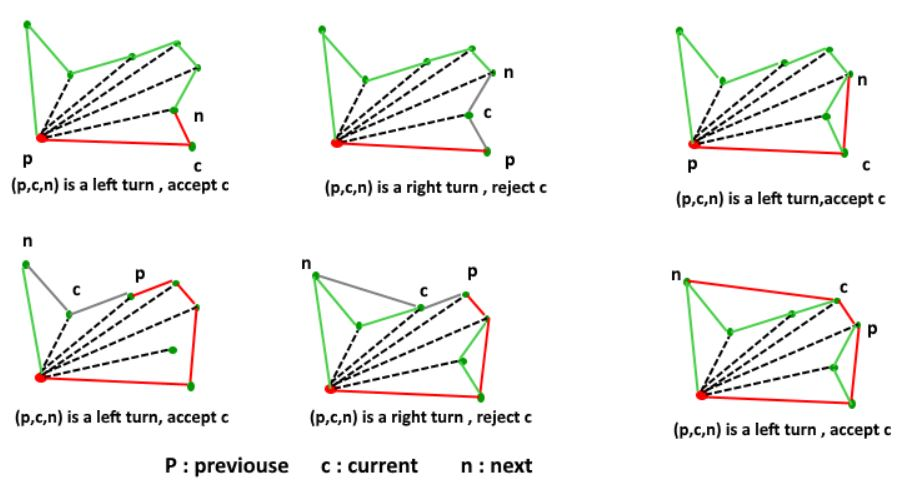
\includegraphics[width=10cm]{graham_scan.jpg}
	\caption{Princip vyhodnocení polohy bodu v metodě Graham Scan [zdroj: 6]}
\end{figure}

\subsubsection{Implementace metody}
\begin{enumerate}
\item Nalezení pivota q:  $ q = min_{\forall p_i \in S} (y_i), q \in H $ 
\item Setřídění bodů dle úhlu s osou x: $ {\forall p_i \in S}$ sort by $ \omega_i = \angle (p_i, q, x)$
\item Při nalezení stejného úhlu: $ \omega_k = \omega_l \rightarrow $ delete the closer point 
\item Vložení pivota a prvního bodu do množiny: $ H \leftarrow q; H \leftarrow p_1$
\item Opakuj pro všechna: $ for j < n $
\item Vyhodnocení polohy bodu: if $ p_j $ vpravo od předešlých bodů $ \rightarrow pop S$
\item V opačném případě přidej bod do konvexní obálky: $ p_{j}  \rightarrow H $
\end{enumerate}

\section{Informace o bonusových úlohách}
V podkapitolách jsou blíže popsány bonusové úlohy kromě algoritmu Graham Scan, ten byl již vysvětlem a popsán v rámci použitých algoritmů. Zároveň není blíže popsán stav kolineárních bodů při metodě Jarvis Scan. Tento stav je specifikován v rámci kapitoly zabývající se algoritmem Jarvis Scan v podkapitole Problematické situace.

\subsection{Automatické generování množin bodů}
Pro tvorbu automatického generování množin bodů je možné zvolit útvar, v němž budou generované body vykresleny. V rámci aplikaci si může uživatel vybrat mezi kruhem, čtvercem, elipsou, gridem, náhodném rozmístění či star shaped útvarem. Veškeré body jsou odsazeny, aby elipsy, které bod reprezentují, nebyly nějakým způsobem oříznuté.

\subsubsection{Circle}
Pro tvorbu kruhu byl nejprve náhodně vygenerován střed kružnice a její poloměr. V závislosti na počtu bodů byl určen středový úhel po sobě jdoucích bodů. Po znalosti těchto hodnot bylo snadné vygenerovat body na kružnici:\\
$ X = X_0 + r * cos(\phi)$ \\
$ Y = Y_0 + r * sin(\phi) $

\subsubsection{Ellipse}
Elipsa byla generována obdobně jako kruh s tím rozdílem, že nebyl generován poloměr, ale hodnota hlavní poloosy (a) a vedlejší poloosy (b). 
$ X = X_0 + a * cos(\phi)$ \\
$ Y = Y_0 + b * sin(\phi) $

\subsubsection{Square}
Při tvorbě čtverce je nejprve vygenerováno náhodné umístění levého horního rohu. Poté je náhodně vypočtena délka hrany. Se znalostí délky hrany jsme schopni určit zbylé vrcholy čtverce a zároveň zobrazit body na hranách. Při generování čtverce je vstupní množství zredukováno tak, aby počet bodů odpovídal počtu nutnému pro zobrazení čtverce. Pro představu - z pěti bodů čtverec nesestavíte, tudíž pokud to je nutné, tak dochází k přepočítání počtu bodů. Na tento fakt je uživatel aplikací upozorněn.

\subsubsection{Star Shaped}
Při tvorbě Star Shaped polygonu je automaticky vygenerován střed a poloosy a, b. Pro polygony typu star shaped je typické, že z jeho středu lze vidět do všech vrcholů. Dva po sobě jdoucí body budou vytvořeny s různou vzdáleností od středu, čímž této podmínky docílíme. Středový úhel mezi dvěma následujícími body bude opět určen v závislosti na vstupnímu množství dat.\\
$ X_i = X_0 + a * cos(\phi)$ \\
$ Y_i = Y_0 + a * sin(\phi) $ \\
$ X_{i+1} = X_0 + b * cos(\phi)$ \\
$ Y_{i+1} = Y_0 + b * sin(\phi) $

\subsubsection{Grid}
Pro tvorbu pravidelné mřížky je zapotřebí, aby vstupní počet bodů byl druhu mocninou nějakého přirozeného čísla. Pokud tato podmínka není splněna, je počet redukován a uživatel je o změně informován. Takovýto případ může nastat například při zadání 18 bodů. Počet je v tomto případě zredukován na 16 a vytvořený grid má velikost 4 x 4. Podobně jako při tvorbě čtverce je vygenerován první bod, od nějž jsou následně zbylé body vypočteny.

\subsubsection{Random}
Body byly náhodně rozmístěny v rámci zobrazovacího okna.

\subsection{Konstrukce striktně konvexních obálek}
Striktně konvexní obálky jsou takové, že po sobě následující 3 body neleží na stejné přímce. V případě vygenerovaného čtverce o sto bodech bude striktně konvexní obálka obsahovat pouze 4 body, a to vrcholy. Pro tvorbu striktně konvexních obálek byla po vygenerování klasických obálek volána funkce na určení pozice bodu vůči linii. Pokud byl následující bod vyhodnocen tak, že leží na orientované úsečce $\overrightarrow{AB}$, bod B byl z množiny odebrán a následně byla testována další trojice bodů. Zároveň bylo nutné odebrat duplicitní body.


\subsection{Konstrukce Minimum Area Enclosing Box}
V rámci bonusových úloh bylo i sestrojení obdélníku s minimální plochou s využitím konvexní obálky. Tvorba takovýchto obdélníků se využívá v kartografii pro detekci tvaru a natočení budov. Případně by se mohla metoda používat v rámci generalizace, zde by však bylo zapotřebí ošetřit, aby výsledná data byla topologicky čistá. Při tvorbě minimálního obdélníku s využitím konvexní obálky se vychází z předpokladu, že nejméně jedna strana obdélníka je kolineární se stranou konvexní obálky. Složitost takovéto konstrukce má časovou náročnost O(n). 

\begin{figure}[h!]
	\centering
	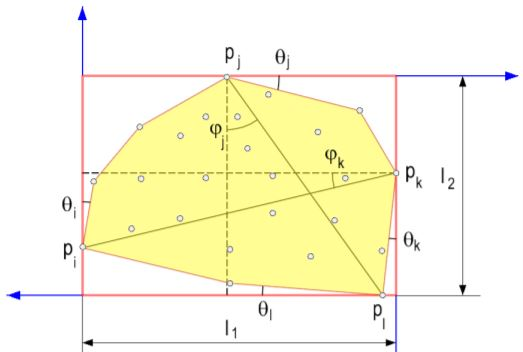
\includegraphics[width=10cm]{mbr.jpg}
	\caption{Princip tvorby Minimum Bounding Rectangle včetně znázornění úhlů a stran, které jsou tímto způsobem také popsány v následné implementaci metody. [zdroj: 5]}
\end{figure}

\subsubsection{Implementace metody}
\begin{enumerate}
\item Inicializuj: $ A_{min} = \infty; rot = 0; \Phi_{sum} = 0$
\item Nalezení Minimum Bounding Rectangle, který se dotýká konvexní obálky v extrémních bodech (min X, max X, min Y, max Y)
\item Výpočet úhlů a plochy: $ \phi_j, \phi_k, A(R)$
\item Vložení vypočtené plochy do minimální: $A_{min} = A$
\item Opakuj dokud: $\Phi_{sum} \textless  {\pi/4}$
\subitem Výpočet úhlů $\Phi_i, \Phi_j, \Phi_k, \Phi_l$ a stran $l_1, l_2$
\subitem Nalezni nejmenší úhel: $\Phi = min(\Phi_i, \Phi_j, \Phi_k, \Phi_l)$
\subitem Otočení obdélníku o úhel $\Phi$
\subitem Výpočet plochy obdélníku a porovnání s dosavadní minimální plochou.
\subitem Při nalezení menší plochy: $A_{min} = A; rot = rot + \Phi; L_1 = l_1; L_2 = l_2$
\subitem $\Phi_{sum} = \Phi_{sum} + \Phi$
\end{enumerate}

\section{Vstupní data}
Vstupními daty je množina bodů, která je vygenerovaná uživatelem. Uživatel může v tomto případě generovat body sám za pomoci kurzoru. Případně je v aplikaci implementována funkce pro automatické generování bodů. Uživatel má navíc možnost vlastní volby, jakým způsobem budou body generovány, zda budou body v kruhu, ve čtverci, elipse či v gridu. \\
\\
Při automatickém generování bodů je nutné nastavit i počet bodů, ze kterých bude daný útvar tvořen. Ne všechny tvary však lze vytvořit z vloženého množství bodů. V případě, že vstup nebude zcela odpovídat zvolenému útvaru, zobrazí se uživateli vyskakovací okno, které upozorní na nevhodný vstup a případnou modifikaci vloženého počtu. Tento případ nastane například při vložení tří bodů, ze kterých by uživatel chtěl vytvořit čtverec. 



\section{Výstupní data}
Výstupem této úlohy je grafická aplikace, ve které jsou vstupní data analyzovány a následně je v závislosti na jejich vzájemně poloze vytvořena konvexní obálka. Konvexní obálku je možné vytvořit čtyřmi způsoby za pomoci nejznámějších algoritmů - Jarvis Scan, Quick Hull, Sweep Line a Graham Scan.\\
\\
Zároveň jsou výstupem data s porovnáním jednotlivých dob výpočtů na různém množství dat. Tyto hodnoty jsou vzájemně porovnány za pomoci tabulek a grafů.

\clearpage
\section{Aplikace}
\begin{figure}[h!]
	\centering
	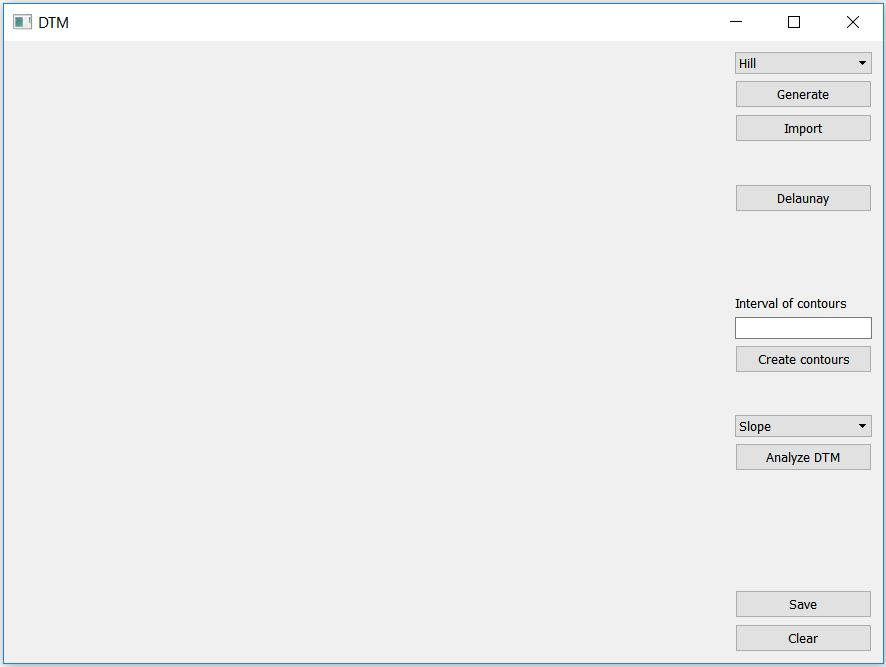
\includegraphics[width=10cm]{vstup.jpg}
	\caption{Zobrazené okno po spuštění aplikace}
\end{figure}

\begin{figure}[h!]
	\centering
	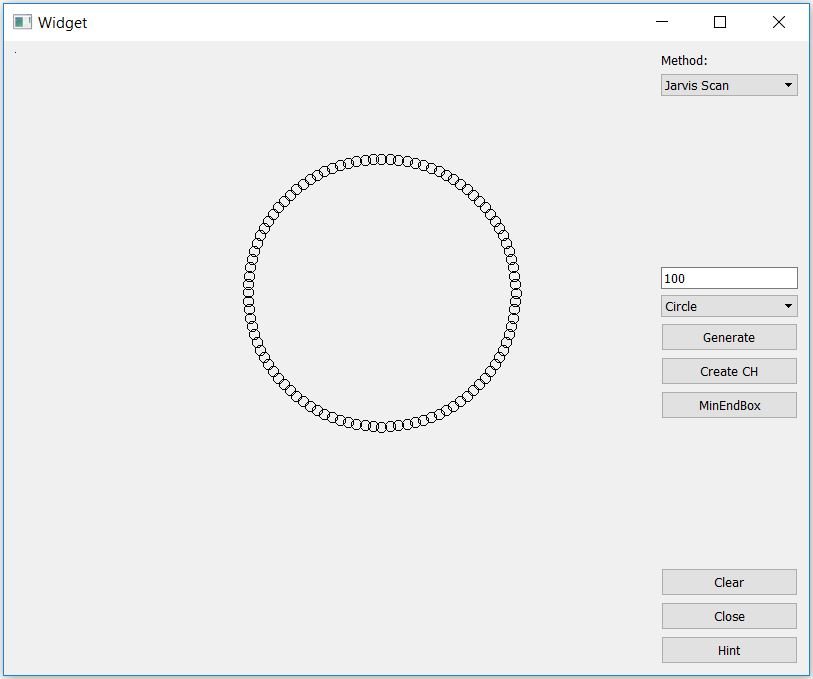
\includegraphics[width=10cm]{circle.jpg}
	\caption{Vygenerované body v kruhu}
\end{figure}

\begin{figure}[h!]
	\centering
	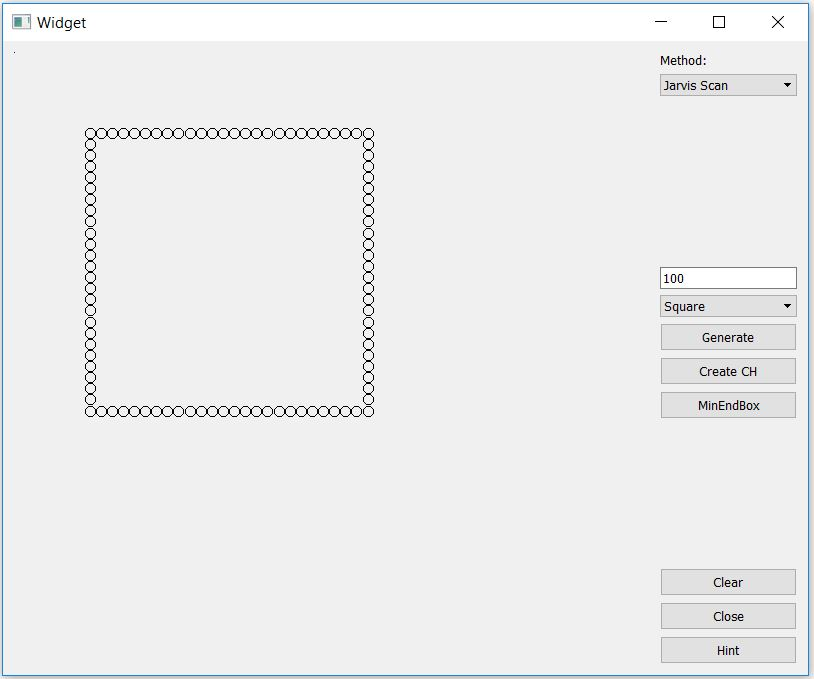
\includegraphics[width=10cm]{square.jpg}
	\caption{Vygenerované body ve čtverci}
\end{figure}

\begin{figure}[h!]
	\centering
	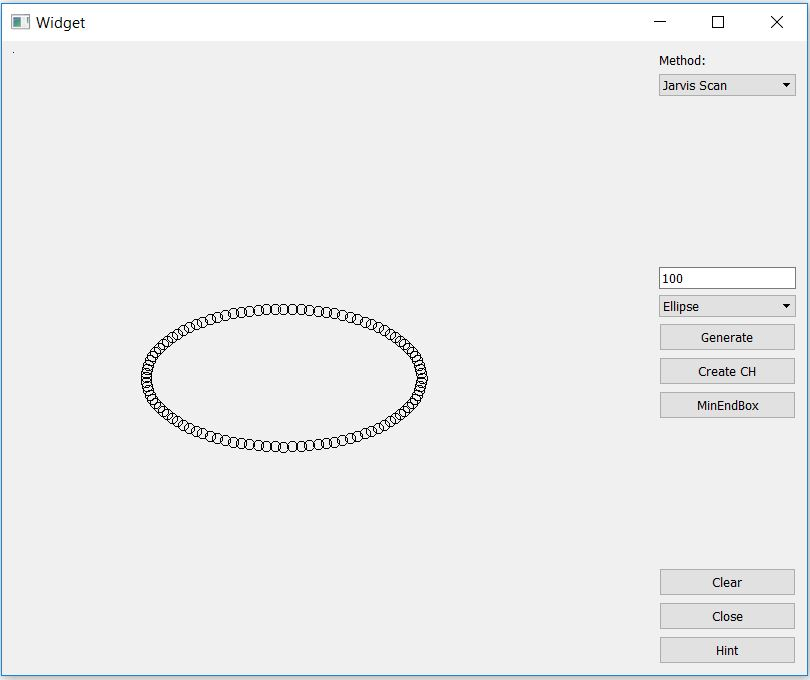
\includegraphics[width=10cm]{ellipse.jpg}
	\caption{Vygenerované body v elipse}
\end{figure}

\begin{figure}[h!]
	\centering
	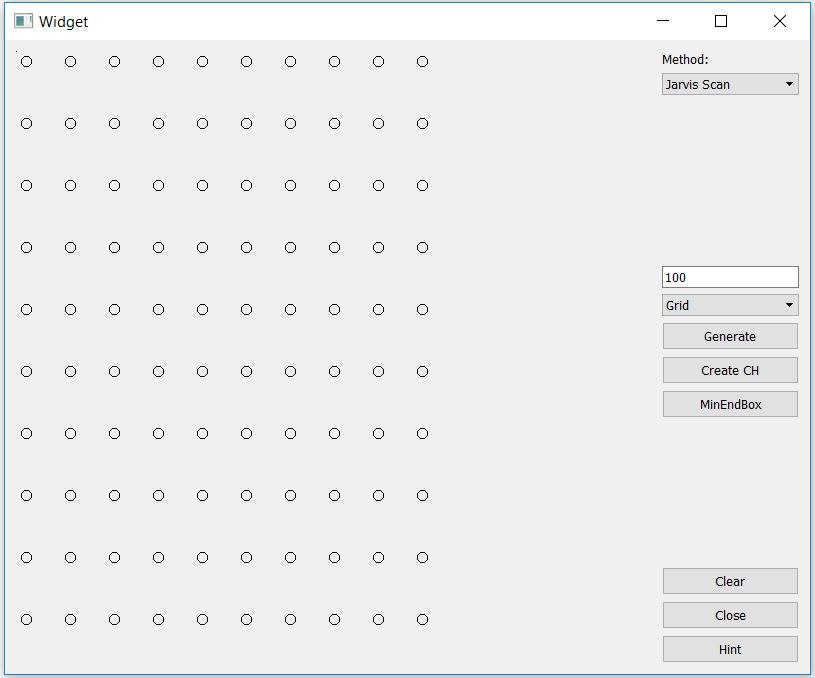
\includegraphics[width=10cm]{grid.jpg}
	\caption{Vygenerované body v pravidelné mřížce}
\end{figure}

\begin{figure}[h!]
	\centering
	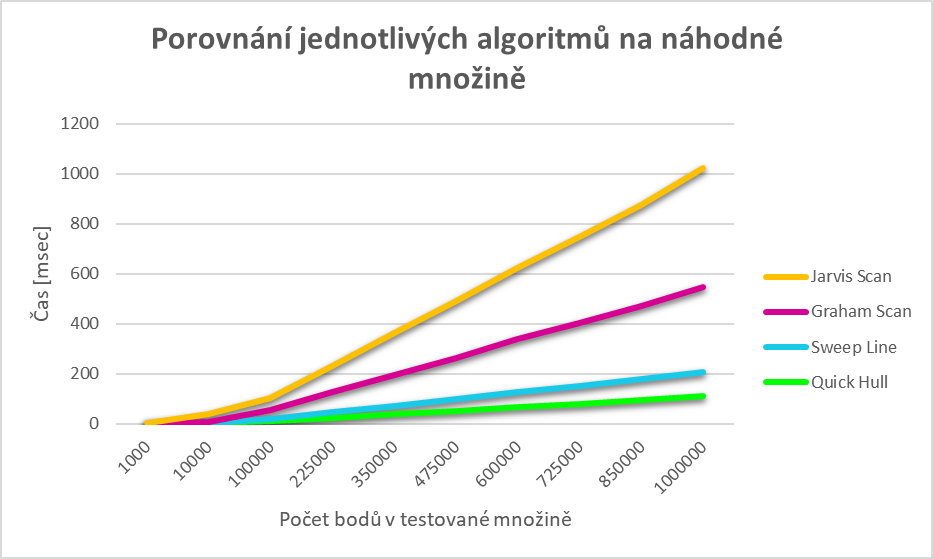
\includegraphics[width=10cm]{random.jpg}
	\caption{Náhodně vygenerované body}
\end{figure}

\begin{figure}[h!]
	\centering
	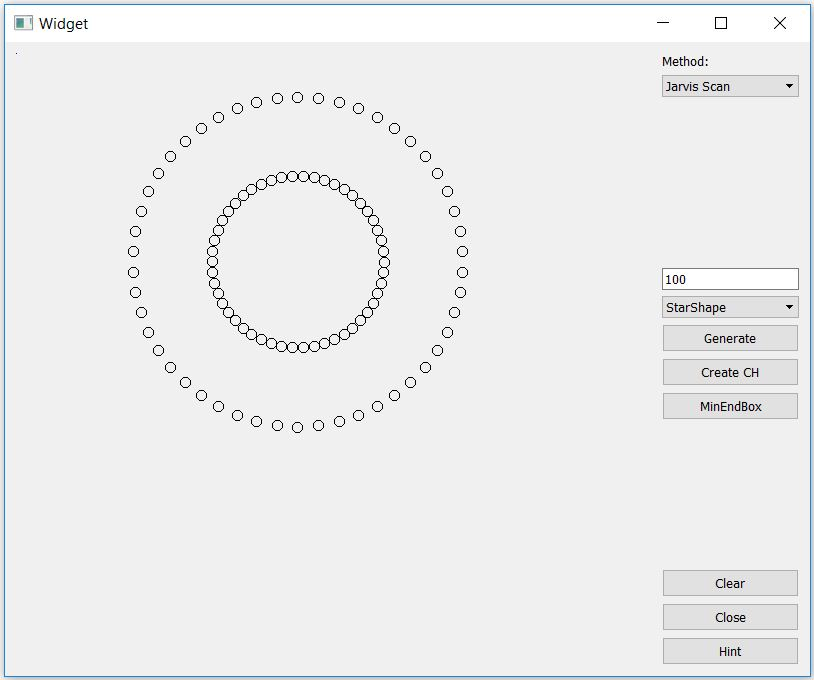
\includegraphics[width=10cm]{star_shaped.jpg}
	\caption{Vygenerované body ve tvaru Star Shaped}
\end{figure}

\begin{figure}[h!]
	\centering
	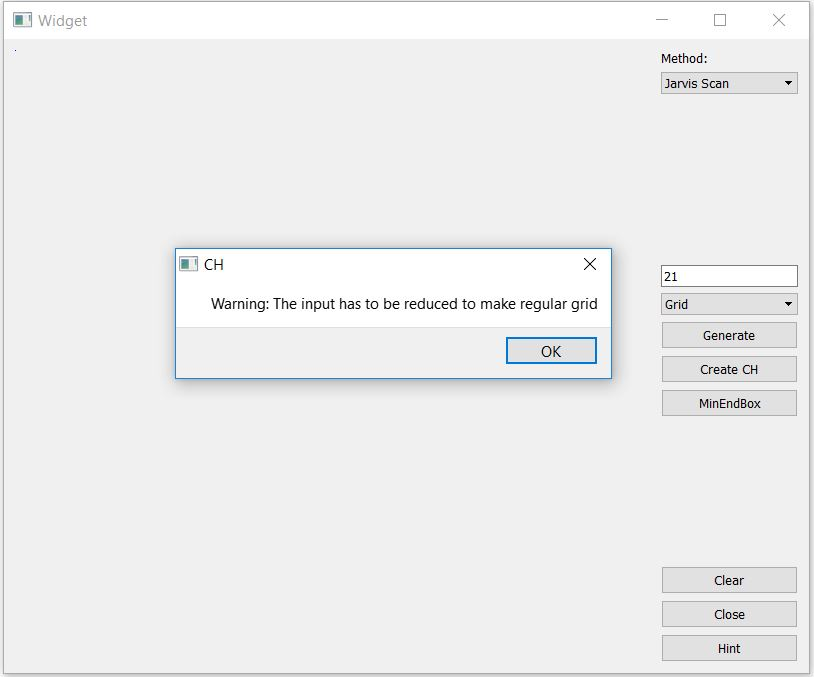
\includegraphics[width=10cm]{warning_grid.jpg}
	\caption{Varování na redukci vloženého počtu bodů při tvorbě gridu }
\end{figure}

\begin{figure}[h!]
	\centering
	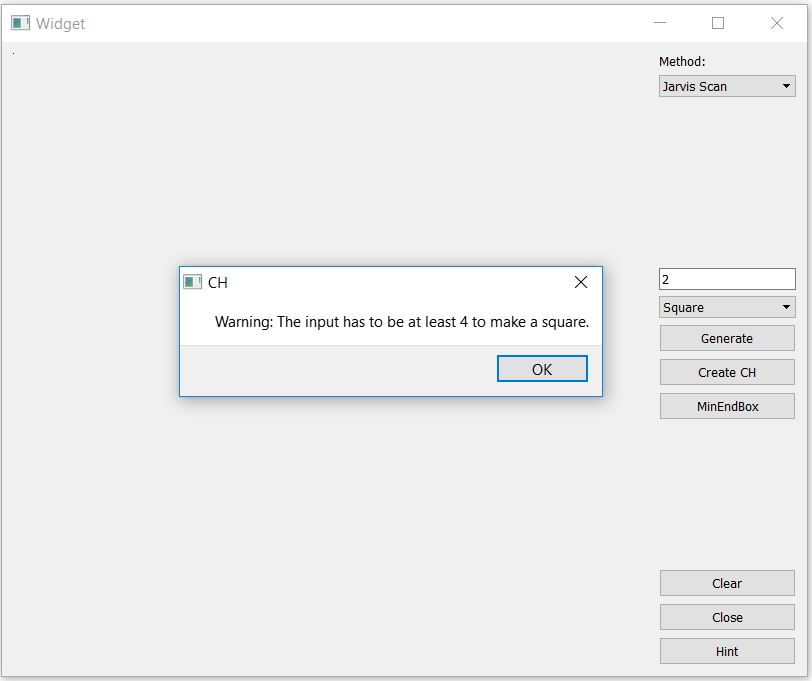
\includegraphics[width=10cm]{warning_square.jpg}
	\caption{Varování při neplatném vstupu při tvorbě čtverce}
\end{figure}

\begin{figure}[h!]
	\centering
	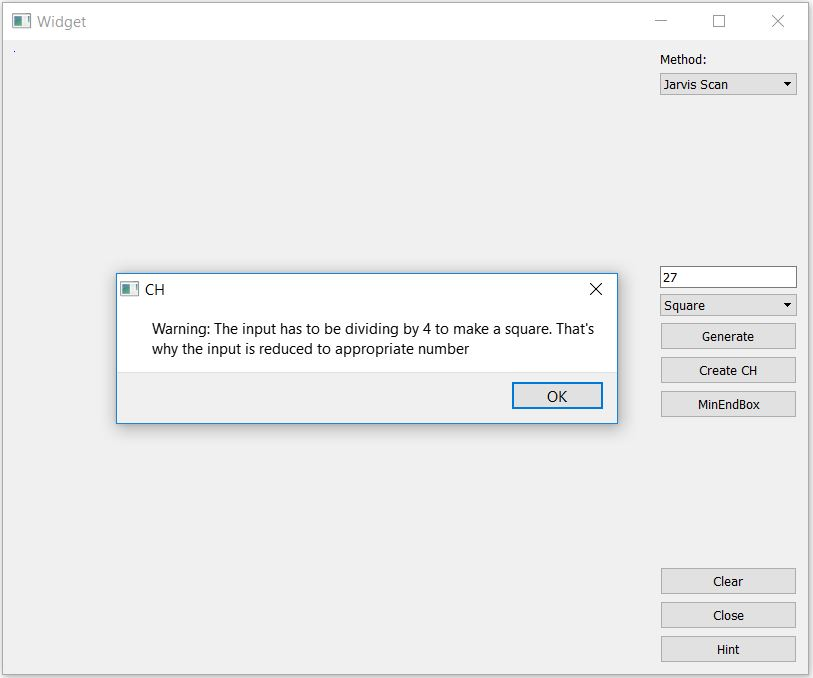
\includegraphics[width=10cm]{warning_square2.jpg}
	\caption{Varování na redukci vloženého počtu bodů při tvorbě čtverce}
\end{figure}

\begin{figure}[h!]
	\centering
	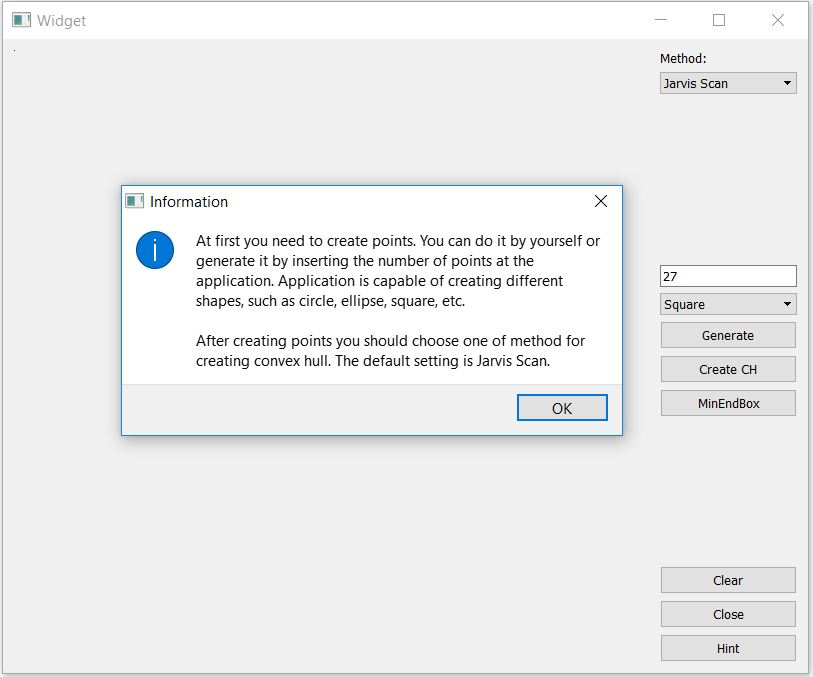
\includegraphics[width=10cm]{hint.jpg}
	\caption{Nápověda, pokud si uživatel nebude jistý, jak v aplikaci postupovat}
\end{figure}

\begin{figure}[h!]
	\centering
	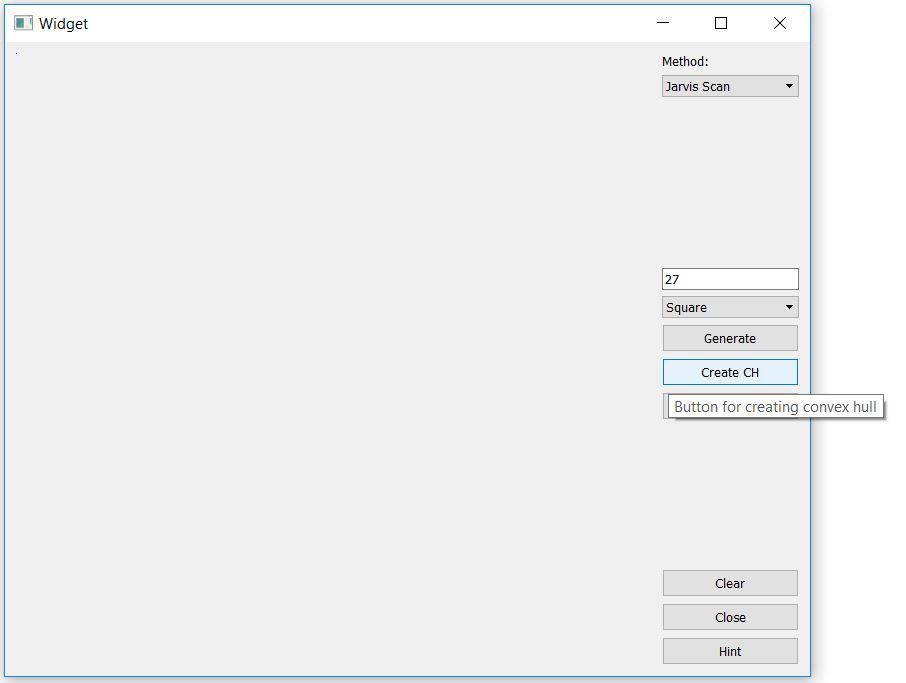
\includegraphics[width=10cm]{tooltip.jpg}
	\caption{Po přiložení kurzoru se zobrazí informace o objektu}
\end{figure}

\begin{figure}[h!]
	\centering
	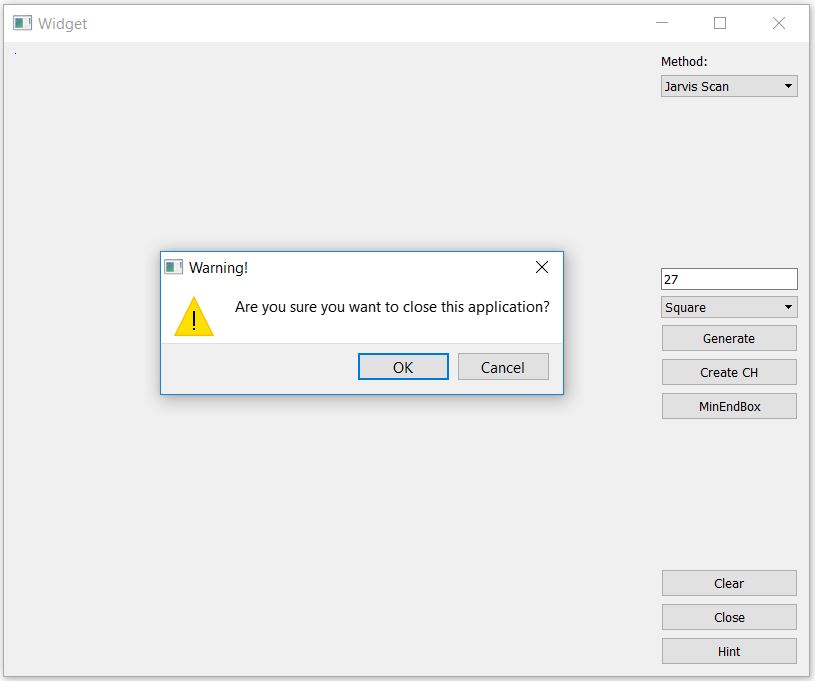
\includegraphics[width=10cm]{close.jpg}
	\caption{Vyskakovací okno při ukončování aplikace}
\end{figure}

\clearpage

\section{Dokumentace}
\subsection{Třídy}
\subsubsection{Algorithms}
Třída Algorithms obsahuje celkem xx metod. Metody jsou určeny pro výpočty použitých algoritmů.
\\

\textbf{double length2Points(QPoint q, QPoint p)}
Metoda jejíž návratová hodnota je typu double vrací velikost spojnice mezi dvěma body.
\\

\textbf{void polygonTransform(QPoint p, QPoint k, QPoint p1, QPoint k1, QPolygon \&pol)}
Metoda je přetížená pro  podobnostní transformaci QPolygon a QLine. Transformační klíč je dán dvěma body se souřadnicemi v obou souřadných soustavách. Body p a k jsou v souřadné soustavě, ze které pochází pol. Body p1 a k1 jsou v souřadné soustavě, do které chceme transformovat. Výsledek transformace přeuloží do proměnné pol.
\\

\textbf{rotateByAngle(QPolygon \&points, double angle)}
Metoda je přetížená pro rotaci QPolygon a QLine. Prvky proměnné pol se pouze rotují podle úhlu angle. Proměnná úhel je v radiánech. Výsledek transformace přeuloží do proměnné pol.
\\

\textbf{TPosition getPointLinePosition(QPoint \&q, QPoint \&a, QPoint \&b)}
\\


\textbf{double get2LinesAngle(QPoint \&p1,QPoint \&p2,QPoint \&p3, QPoint \&p4)}
\\


\textbf{QPolygon CHJarvis (vector\textless QPoint \textgreater \&points)}
Metoda pro výpočet konvexní obálky nad vektorem bodů metodou Jarvis Scan. Metoda vrácí konvexní obálku s typem QPolygon.
\\

\textbf{QPolygon QHull (vector\textless QPoint \textgreater \&points)}
Metoda pro výpočet konvexní obálky nad vektorem bodů metodou Quick Hull. Metoda vrácí konvexní obálku s typem QPolygon.
\\

\textbf{void qh (int s, int e, vector\textless QPoint \textgreater \&p, QPolygon \&h)}
Pomocná metoda pro rekurzi v metodě Qhull. Na vstupu jsou indexi bodů s a e, které určují přímku, podle níž se určí zda bod p patří do konvexní obálky h a nebo ne. Metoda nic nevrací, pouze ukládá body, které patří do konvexní obálky.
\\

\textbf{void minimumAreaEnclosingBox (QPolygon \&ch, QPolygon \&rectangle, QLine \&direction)}
Metoda pro výpočet hlavních směrů budovy. Na vstupu je konvexní obálka ch a prázdné proměnné rectangle a direction. Do rectangle se uloží minimální ohraničující obdélník a do direction hlavní směr budovy.
\\

\subsubsection{Draw}
Třída Draw obsahuje celkem xx metod. Metody jsou určeny pro generování a vykreslování proměných.
\\

\textbf{void paintEvent(QPaintEvent *e)}
Metoda slouží k vykreslení vytvořených, generovaných bodů a zobrazení výsledků použitých algoritmů.
\\

\textbf{void mousePressEvent(QMouseEvent *e)}
Po stisknutí levého tlačítka myší na zobrazovací okno, metoda uloží bod se souřadnicemi místa kliknutí.
\\

\textbf{void clearCanvas()}
Metoda slouží k vymazání proměnných a k překreslení
\\

\textbf{std::vector\textless QPoint \textgreater generateGrid(int n)}
Metoda generuje pravidelnou mřížku. Na vstupu je počet generovaných bodů. Návratová hodnota je vektor bodů.\\
\\
\textbf{std::vector\textless QPoint \textgreater generateRandomPoints(int n)}
Metoda generuje náhodné body. Na vstupu je počet generovaných bodů. Návratová hodnota je vektor bodů.\\
\\
\textbf{std::vector\textless QPoint \textgreater generateStarShape(int n)}
Metoda generuje body do tvaru hvězdy. Na vstupu je počet generovaných bodů. Návratová hodnota je vektor bodů.\\
\\
\textbf{std::vector\textless QPoint \textgreater generateSquare(int n)}
Metoda generuje body do tvaru čtverce. Na vstupu je počet generovaných bodů, změna v počtu bodů se projení s násobkem čtyř. Návratová hodnota je vektor bodů.\\
\\
\textbf{std::vector\textless QPoint \textgreater generateEclipse(int n)}
Metoda generuje body do tvaru elipsy. Na vstupu je počet generovaných bodů. Návratová hodnota je vektor bodů.\\
\\
\textbf{std::vector\textless QPoint \textgreater generateCircle(int n)}
Metoda generuje body do tvaru kruhu. Na vstupu je počet generovaných bodů. Návratová hodnota je vektor bodů.\\
\\
\textbf{void setCH(QPolygon ch\_)}
Metoda slouží pro převod konvexní obálky do vykreslovacího okna.\\
\\
\textbf{setRectangle(QPolygon rectangle\_)}
Metoda slouží pro převod minimální ohraničujícího obdélníku do vykreslovacího okna.\\
\\
\textbf{setDirection(QLine direction\_)}
Metoda slouží pro převod hlavního směru budovy do vykreslovacího okna.\\
\\
\textbf{setPoints(std::vector\textless QPoint \textgreater points\_)}
Metoda slouží pro převod vektoru bodů do vykreslovacího okna.\\
\\
\textbf{std::vector\textless QPoint \textgreater getPoints()}
Metoda slouží pro převod vektoru bodů z vykreslovacího okna.\\
\\
\textbf{QPolygon getConvexHull()}
Metoda slouží pro převod konvexní obálky z vykreslovacího okna.\\
\\
\subsubsection{SortByXAsc}
Třída SortByXAsc slouží k porovnání souřadnic v ose x.\\
\\

\textbf{bool operator()(QPoint \&p1, QPoint \&p2)}
Přetížený operátor () vrátí bod s větší souřadnicí x z dvojice bodů.\\
\\

\subsubsection{sortByYAsc}
Třída SortByXAsc slouží k porovnání souřadnic v ose y.
\\

\textbf{bool operator()(QPoint \&p1, QPoint \&p2)}
Přetížený operátor () vrátí bod s větší souřadnicí y z dvojice bodů.
\\

\subsubsection{Widget}


\textbf{void on\_pushButton\_clicked()}
Při stisknutí tlačítka Create CH se volají metody třídy Algorithms dle metody vybrané v comboboxu.
\\

\textbf{void on\_generate\_clicked()}
Při stisknutí tlačítka Generate se volají metody třídy Draw dle metody vybrané v comboboxu.
\\

\textbf{void on\_pushButton\_2\_clicked()}
Při stisknutí tlačítka Clear se zavolá metoda třídy Draw clearCanvas.
\\

\textbf{void on\_minimumAreaEnclosingBox\_clicked()}
Při stisknutí tlačítka MinEndBox se nad konvexní obálkou zavolá metoda třídy Algorithms minimumAreaEnclosingBox.
\\

\clearpage
\section{Závěr}
V rámci úlohy byla vytvořena aplikace, která je schopna na vygenerovaných bodech zkonstruovat konvexní obálku. Zároveň je v rámci aplikace možné náhodně vygenerovat téměř libovolné množství bodů do určitého tvaru. Na výběr je poměrně široké spektrum běžných tvarů, což jistě uživatel ocení.

\section{Náměty na vylepšení}
\subsection{Graham Scan}
V algoritmu Graham Scan pro výpočet konvexní obálky je po zamyšlení zřejmě použit příliš složitý postup výpočtu úhlu s osou x. Zároveň víme, že velikosti směrnic budou vždy dosahovat hodnot od 0 do 180, neboť se jedná o úhel mezi pivotem a osou X. Tudíž některé řádky týkající se určení kvadrantů jsou zbytečné.

\subsection{Generování množin bodů}
Při tvorbě generování gridu napadla autory myšlenka, že by se body generovaly v některém ze známých kartografických zobrazení. Z bakalářského studia znají velké množství zobrazovacích rovnic, pomocí nichž by se body zobrazovaly. Zajímavé rozmístění by měla zejména kuželová zobrazení. Při zobrazení bodů v rámci některého kartografického zobrazení by výsledná konvexní obálka představovala celý svět, případně polokouli, záleželo by na typu zvoleného zobrazení.

\subsection{Testování algoritmů}
V rámci této úlohy bylo provedeno několik testování nad odlišným množstvím bodů a na jejich odlišném zobrazení. Časově bylo testování poměrně náročné, za úvahu jistě stojí popřemýšlení, zda by nebylo výhodnější vytvořit takovou funkci, která by pro předem definované tvary a množství bodů sama provedla testování. Zároveň obsahuje platforma Qt i knihovnu grafů, časová úspora by tedy byla velmi výrazná.



\clearpage
\section{Reference}

\begin{enumerate}
\item  MARTÍNEK, Petr. Konvexní obálka rozsáhlé množiny bodů v E\^d [online][cit. 31.10.2018]. \\
Dostupné z: http://graphics.zcu.cz/files/86\_BP\_2010\_Martinek\_Petr.pdf  \\

\item Convex Hulls: Explained. [online][cit. 31.10.2018]\\
Dostupné z: https://medium.com/@harshitsikchi/convex-hulls-explained-baab662c4e94\\

\item Convex-hull mass estimates of the dodo (Raphus cucullatus). [online][cit. 31.10.2018]\\
Dostupné z: https://www.semanticscholar.org/paper/Convex-hull-mass-estimates-of-the-dodo-(Raphus-of-a-Brassey-O\'Mahoney/12e07d3b712561cad16501ac8096120e14901eb8

\item GeeksforGeeks: Convex Hull - Set 1 (Jarvis's Algorithm or Wrapping. [online][cit. 5.11.2018]\\
Dostupné z: https://www.geeksforgeeks.org/convex-hull-set-1-jarviss-algorithm-or-wrapping/

\item  BAYER, Tomáš. Geometrické vyhledávání [online][cit. 5.11.2018]. \\
Dostupné z: https://web.natur.cuni.cz/~bayertom/images/courses/Adk/adk4.pdf  \\

\item GeeksforGeeks: Convex Hull - Set 2 (Graham Scan). [online][cit. 12.11.2018]\\
Dostupné z: https://www.geeksforgeeks.org/convex-hull-set-2-graham-scan/



\end{enumerate}
\end{document}



 